\section{Concentric rings}
\label{sec:double_rings}
This section shall discuss the scattering properties of a double-ring structure as depicted in \Cref{fig:double_ring_sketch}. 
The geometry consists of a substrate layer sandwiched between two concentric metallic rings of outer radii $R_{1},\,R_{2}$ with widths $w_1,\,w_2$ and a metallic ground plane. The rings, substrate and the metallic ground plane are parallel to the $xy$-plane and stacked in $z$-direction.
The rings and the ground plane are chosen to possess the same thickness of $l_z^{\mathrm{R}}$ in $z$-direction, whereas the substrate layer, which separates the ground plane and the rings, measures $l_z^{\mathrm{S}}$.
The geometry is periodic in both, $x$- and $y$-direction with periodicity $L_\mathrm{x}^\mathrm{UC}$ and $L_\mathrm{y}^\mathrm{UC}$, respectively. Therefore the description of one unit cell is sufficient to discuss the scattering properties of the structure.

Fig. \Ref{fig:artist_view} shows an artist's view of the suggested geometry. Suppose we want to design a metamaterial based on the introduced unit cell which absorbs electromagnetic waves of two different frequencies $f_1$ and $f_2$. How should we choose the size of the unit cell, the layer thicknesses and the ring dimensions? 

It's quite natural that each ring can be capable of supporting circulating currents with a certain fundamental frequency and their corresponding higher harmonics. The radius of the ring sets the resonance frequencies and if we think of the gap between the ground plane and the rings as a resonator the following dependency between the radius $R_i$ of a ring and its fundamental frequency $f_i$ can be guessed from dimensional analysis:
\begin{equation}
R_i \propto \frac{c}{f_i}.
\label{eqn:radii}
\end{equation}
In \cref{eqn:radii} $c$ denotes the speed of light -- not necessarily its vacuum value, $c_0$. The constant of proportionality follows from physical reasoning. 

An impinging wave of frequency $\omega = 2\pi f$ will induce an electrical current in each of the rings. If the thickness of the substrate is smaller than the wavelength the metallic backing plane acts as if the ring-currents would interact with their mirror images. The situation which occurs is that $z$-directed electric fields build up, which are confinened between each ring and the ground plane.
, where $n^\mathrm{S}$ is the (for the moment real) refractive index of the substrate. It follows, that the 
length scale which enters \cref{eqn:radii} should be the length of the ring-resonator, $2\pi R_i n^\mathrm{S}$. From this consideration we end up with the dependency
\begin{equation}
R_i = \frac{c_0}{2 n^\mathrm{S}\pi f_i}
\label{eqn:radii_precise}
\end{equation}
between the radius of a ring and its resonant frequency.

If we decide to design an absorber operating at the two commonly used wifi frequencies $f_1=2.4$ GHz and $f_2=5.2$ GHz and assume a refractive index of $n^\mathrm{S}\approx 2$ (an estimate of the refractive index of FR4, a commonly used material in printed circuit boards), \cref{eqn:radii_precise} predicts radii of $R_1\approx10$ mm and $R_2\approx 4.6$ mm. We could further reduce the parameter space by choosing a square unit cell with $L^\mathrm{UC}_\mathrm{x}=L^\mathrm{UC}_\mathrm{y}=L^\mathrm{UC}\gtrsim 2R_1$. By this choice we maximize the number of absorbing rings in the $xy$-plane without shortcutting neighboring rings.

At this point there are still some free parameters, namely the widths $w_1, w_2$ of the rings and the thickness of the substrate. Furthermore it's a priori not clear, whether the radii estimated by \cref{eqn:radii_precise} are to be unterstood as outer, inner or some kind of mean radius.

Since we want to design an absorber which can be manufactured by PCB techniques, we are quite limited in the choice of the substrate and the available board thicknesses. Lets choose the common value of $l_z^\mathrm{S}=2$ mm for the FR4 substrate layer. Literature values for the real part of the relative permittivity of FR4, $\epsilon_\mathrm{r}'$ vary between $4.1$ and $4.6$ and the "real" permittivity probably underlies temporal variations due to fabrication. The dielectric losses are usually specified to be in the range $\tan \delta=0.01--0.02$, where the loss tangent $\tan\delta=\epsilon_\mathrm{r}''\epsilon_\mathrm{r}'$ measures the ratio of the imaginary over the real part of the permittivity for a dielectric material. As a first starting point, we will use $\epsilon_\mathrm{r}=4.6$ and $\tan\delta = 0.02$. Later on, a comparison with experimentally obtained reflection coefficients will show, whether those values should be adjusted.

The copper parts of our structure will enter the simulation by setting their conductivity to $\sigma=56\times 10^6$ S/m. This corresponds to a purely imaginary relative permittivity $\epsilon_\mathrm{r}= \imag \sigma$.

\begin{figure}
\centering
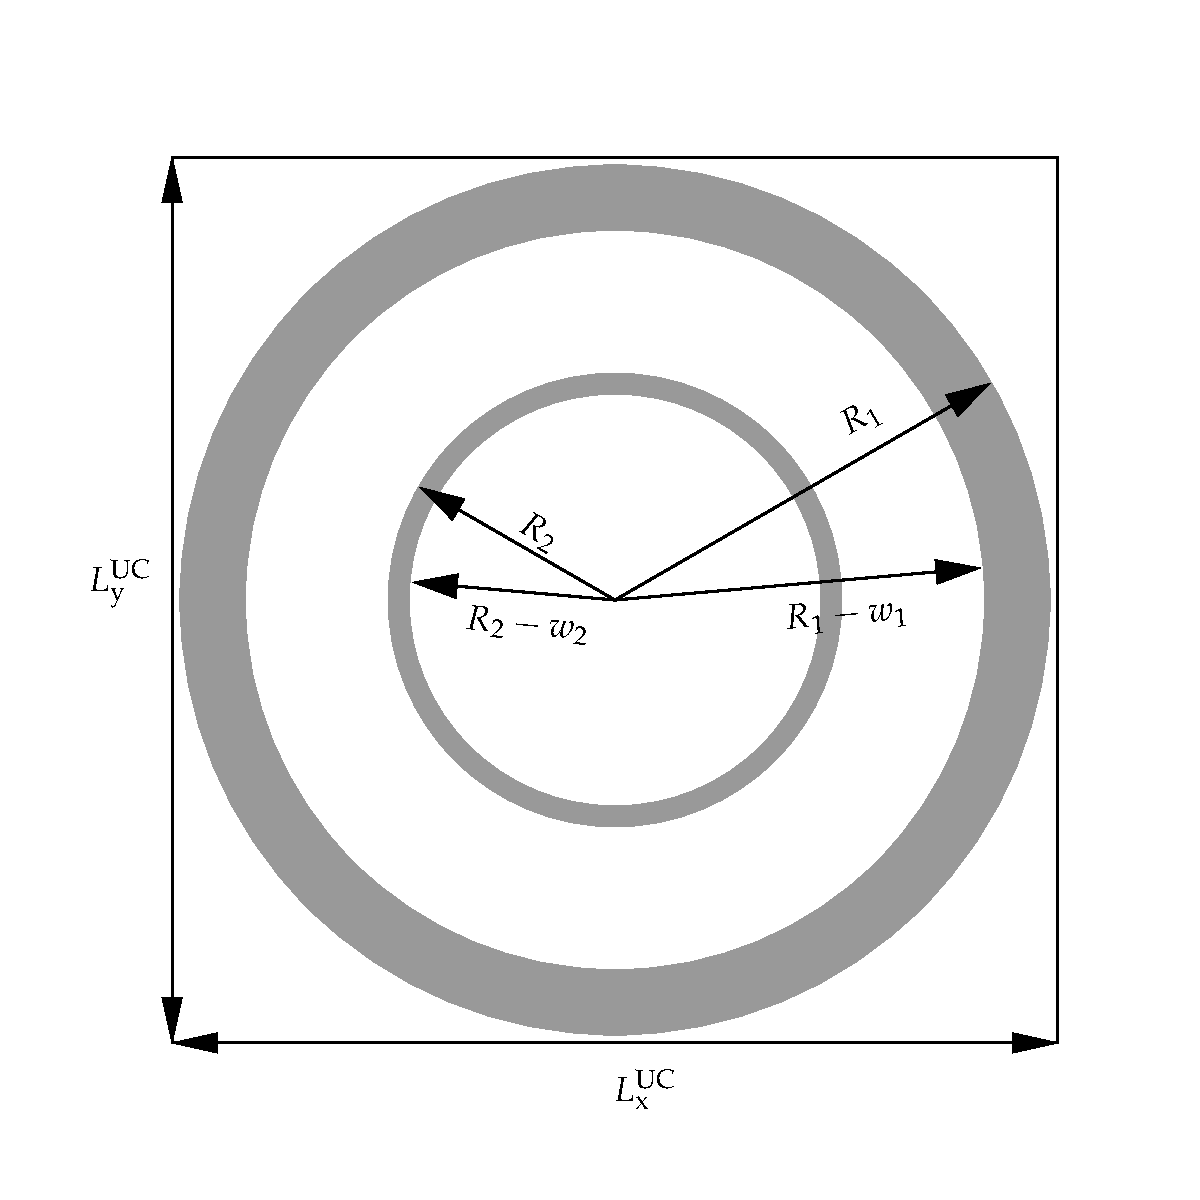
\includegraphics[width=0.75\linewidth]{./media/double_ring_sketch.pdf}
\caption{Two concentric rings of outer radii $R_1$, $R_2$ with widths $w_1$, $w_2$ constitute a metamaterial unit cell with edge lengths of $L_\mathrm{x}^\mathrm{UC}$, $L_\mathrm{y}^\mathrm{UC}$ in $x$- and $y$-direction.}
\label{fig:double_ring_sketch}
\end{figure}

\begin{figure}
\centering
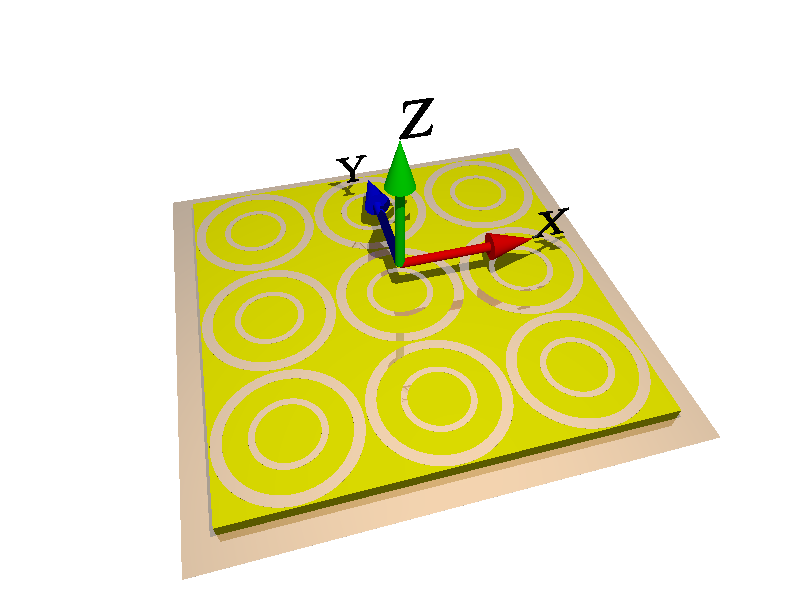
\includegraphics[width=0.75\linewidth]{./media/double_rings.png}
\caption{An artist's view of the suggested metamaterial absorber consisting of a FR4 substrate (yellow) sandwiched between concentric copper rings and a copper backing plane.}
\label{fig:artist_view}
\end{figure}

\subsection{Parameter studies}
In order to find out how the various parameters influence the absorption properties this chapter discusses some numerical results for the reflection parameter $S_{11}$.
In \capFref{fig:w1_sweep} the absolute value of $S_{11}$ as a function of frequency is plotted for a fixed outer ring radius of $R_1=9.8$ mm but changing width $w_1$. As we can see there are several additional drops in the scattering parameter including the desired peaks at about $2.4$ and $5.2$ GHz. Since the $5.2$ GHz peak is contributed by the smaller ring, changing the width of the larger ring does hardly influence the scattering behaviour at resonance of the smaller ring. However, in the frequency range $15<f<20$ GHz a shift to higher frequencies is observed upon an increase of $w_1$. 

\begin{figure}
\centering
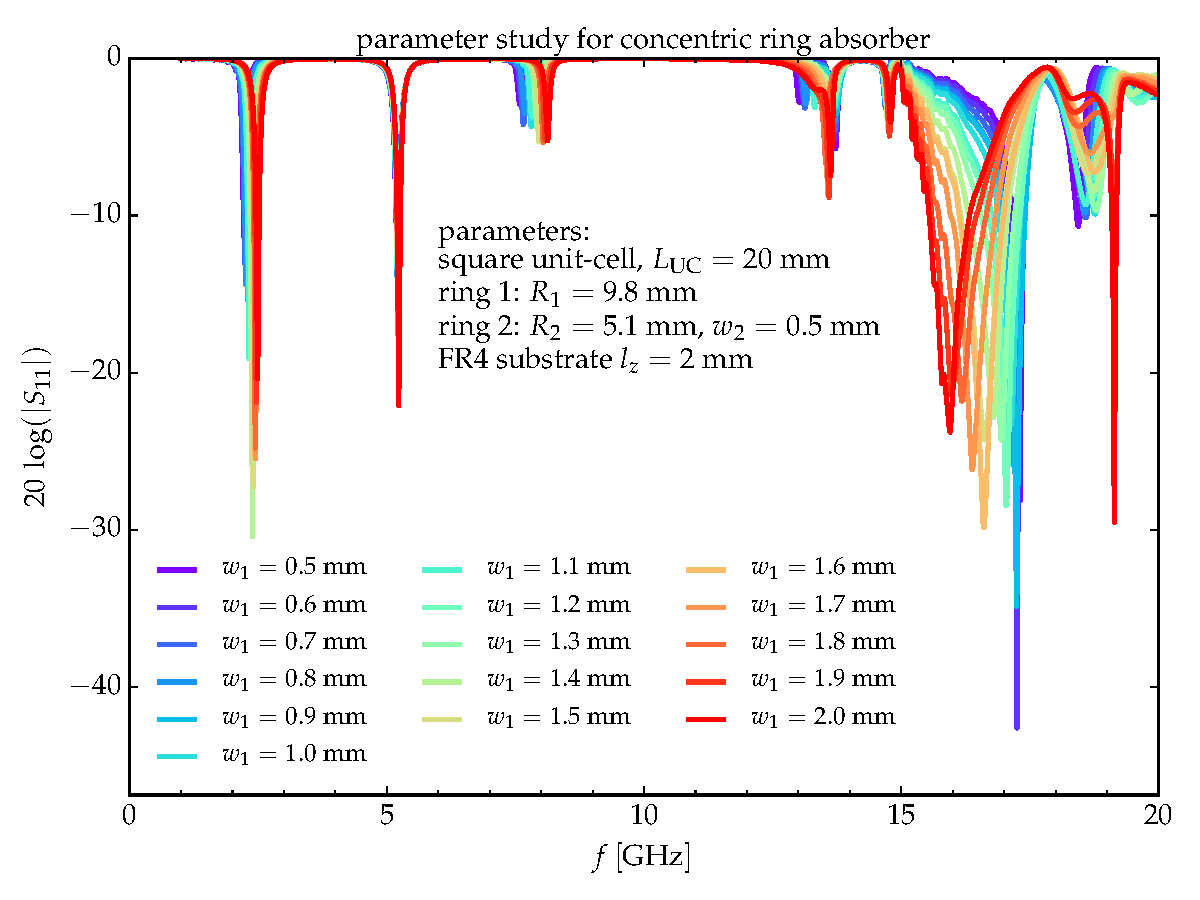
\includegraphics[width=0.75\linewidth]{./media/dual-wifi_absorber_w1.pdf}
\caption{Influence of the larger ring width upon the scattering properties of the concentric ring metamaterial.}
\label{fig:w1_sweep}
\end{figure}

\begin{figure}
\centering
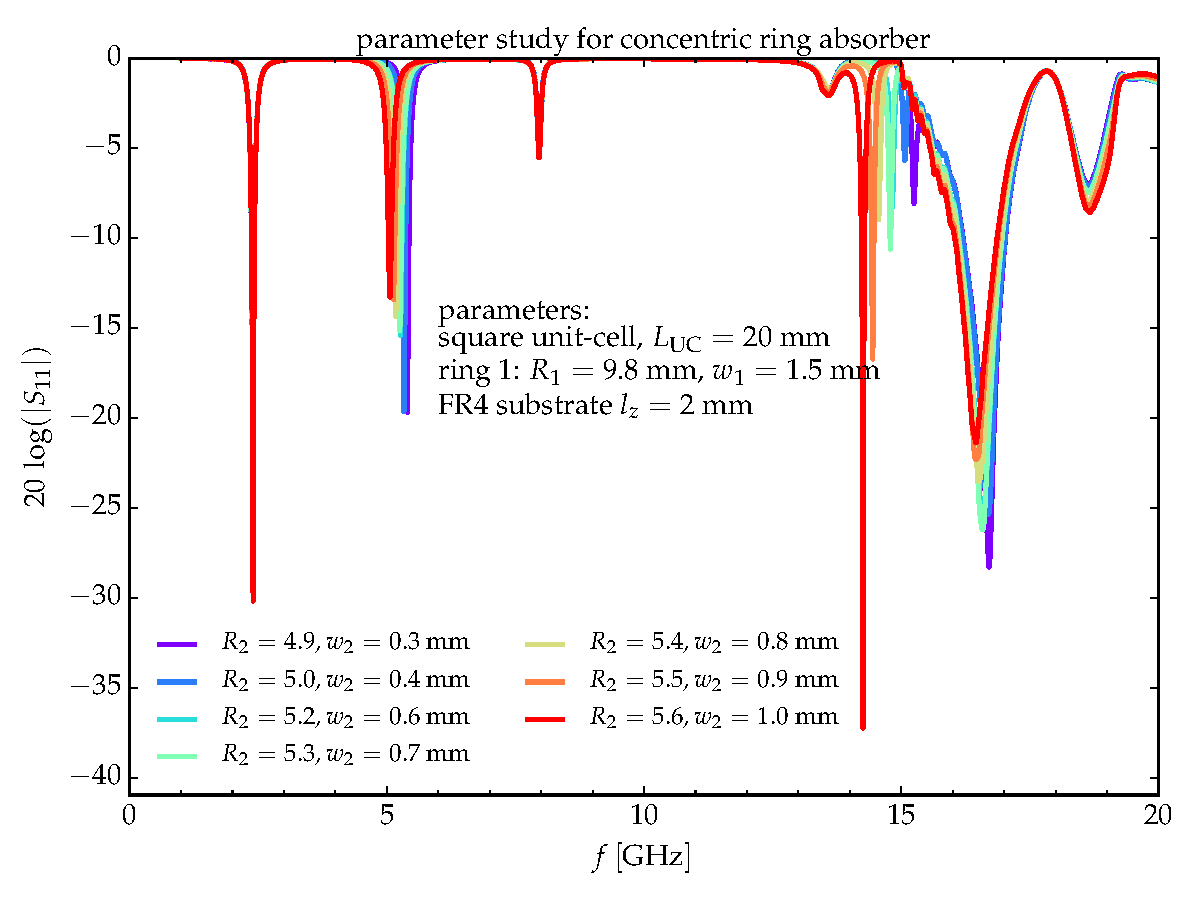
\includegraphics[width=0.75\linewidth]{./media/dual-wifi_absorber_w2.pdf}
\caption{Influence of the smaller ring width upon the scattering properties of the concentric ring metamaterial. In contrast to the study of \Cref{fig:w1_sweep} not the outer, but the inner radius is kept at the value $R_{2i}=4.6$ mm.}
\label{fig:w2_sweep}
\end{figure}

As we would expect a variation of the width of the smaller ring follows the analogous reasoning. \capFref{fig:w2_sweep} exemplifies this behaviour and depicts the absolute value of $S_{11}$ as a function of frequency for a fixed inner ring radius of $R_{2i}=4.6$ mm but changing width $w_2$. Since this time a second peak, namely the one at approximately $8$ GHz doesn't show a dependence upon $w_2$ we can conclude it is associated to a higher harmonic, $f\approx3f_1$, of the larger ring. 

Since in \Cref{fig:w2_sweep} the outer radius of the smaller ring is varied we can conclude, that its neither the inner nor the outer ring radius, but something in between, which enters \cref{eqn:radii_precise}.

To discriminate the influence of both rings \Cref{fig:single_double_rings} shows the absolute value of the scattering parameter of two isolated rings (solid color lines) and the concentric ring configuration (dashed black line) as a function of frequency. Which resonance is caused by which ring can be clearly seen. Aside from that, it can be observed, that the absorption at the second and third resonance is higher for the concentric configuration as compared to the isolated rings.

\begin{figure}
\centering
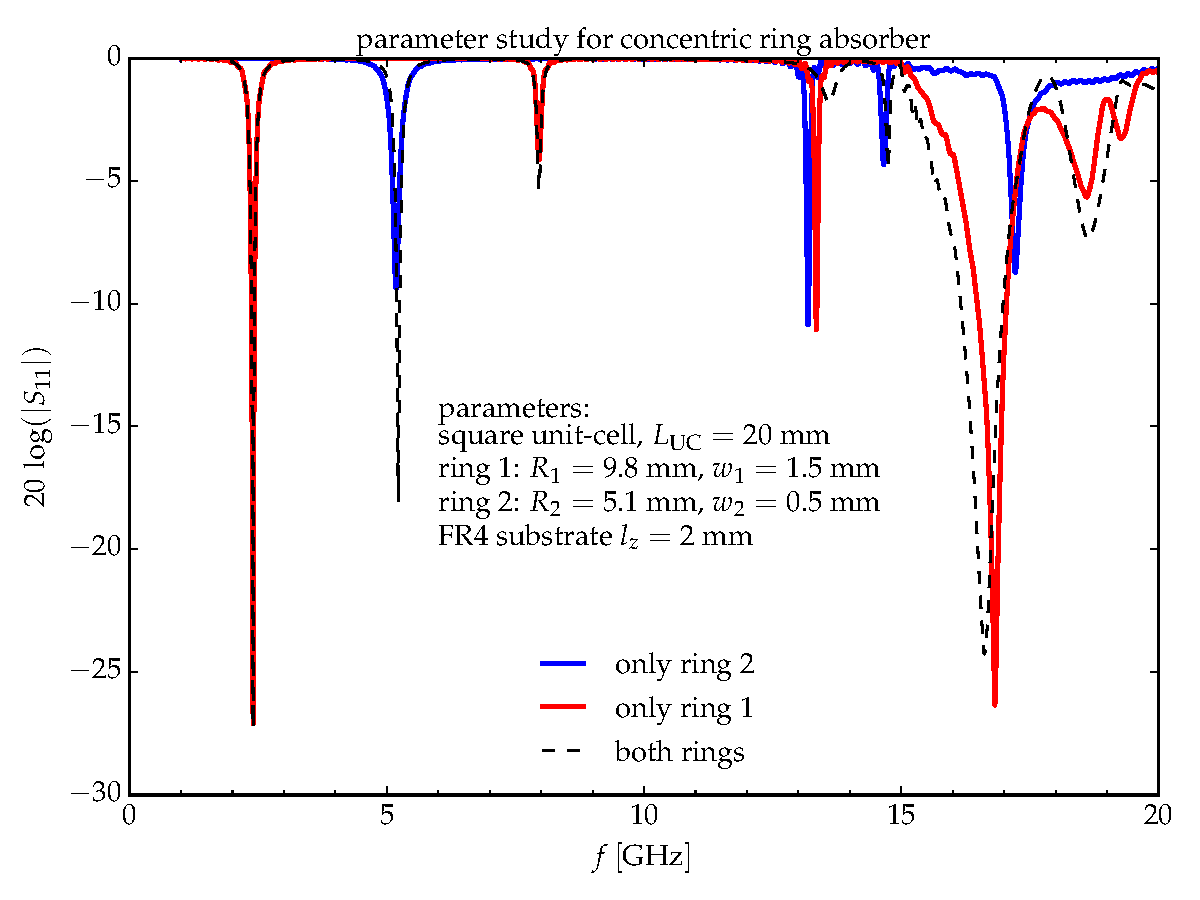
\includegraphics[width=0.75\linewidth]{./media/wifi_absorber_single_double_rings.pdf}
\caption{Comparision of $|S_{11}|$ for an isolated ring 1 with $R_1=9.8$ mm, $w_1=1.5$ mm (red solid), ring 2, $R_2=5.1$ mm, $w_2=0.5$ mm (blue solid) and the concentric configuration (black dashed), where both rings are present.}
\label{fig:single_double_rings}
\end{figure}

To study how the size of the unit-cell influences the position of the absorption 
minima of the double-ring absorber, \Cref{fig:LUC} shows the position of the two first absorption maxima at about $f_1\approx2.7$ GHz and $f_2\approx 5.5$ GHz as a function of the size of the unit cell, $L^\text{UC}$.
\begin{figure}
\centering
\includegraphics[width=0.75\linewidth]{./media/Einfluss_LUC.pdf}
\caption{Simulated position of the first two absorption maxima of a double ring absorber with $R_1=9.8$ mm, $w_1=1.5$ mm, $R_2=5.1$ mm, $w_2=0.5$ mm and $l_z^\mathrm{FR4}=2$ mm as a function of the size of the unit-cell size. Metallic parts are chosen to be copper and FR4 is supposed to possess $\Re\left(\epsilon_\mathrm{r}\right)=4.1$ and a loss tangent of $\tan\delta = 0.015$.}
\label{fig:LUC}
\end{figure}

What can be observed is that as the size of the unit cell grows, the absorption frequency which can be attributed to the larger ring, suffers a shift to higher frequencies. Since this shift tends to saturate as the distance of the outer ring to its neighbours becomes comparable to the ring radius, we can say that a stronger coupling of neighbouring unit cells leads to an increase of the resonance frequency of the larger ring, whereas the resonance frequency of the smaller ring does not show a significant dependence on the size of the unit cell. This is probably the case since $L^\mathrm{UC}/2 R_2\gtrsim 1.8$ even for the smallest unit cell with $L^\mathrm{UC}=20$ mm, where the beginning of the saturation in \Cref{fig:LUC} is way back. The "stepping" which can be observed is due to a finite numerical resolution in frequency.

What is of interest, too is the magnitude of the absorption at the two resonant frequencies as the unit cell grows. \capFref{fig:LUC_absS11} shows this dependency.

\begin{figure}
\centering
\includegraphics[width=0.75\linewidth]{./media/Einfluss_LUC_absS11.pdf}
\caption{Simulated ratio of $|S_{11}(\mathrm{UC})|/|S_{11}(L^\mathrm{UC}=20\,\mathrm{mm})|$ for the first two absorption maxima of a double ring absorber with $R_1=9.8$ mm, $w_1=1.5$ mm, $R_2=5.1$ mm, $w_2=0.5$ mm as a function of the size of the a-dimensional parameter $\eta = L^\mathrm{UC}$. Metallic parts are chosen to be made of copper and FR4 is supposed to possess $\Re\left(\epsilon_\mathrm{r}\right)=4.1$ and a loss tangent $\tan\delta = 0.015$.}
\label{fig:LUC_absS11}
\end{figure}


Another important question concerns the impact of the losses taking place in the substrate. \capFref{fig:tand_fi_41} therefore shows the positions of the first two frequencies with minimal $S_{11}$ as a function of $\tan\delta$ of the FR4 substrate at fixed real part $\epsilon_\mathrm{r}^\text{FR4}=4.1$.
It can be observed, that the loss in the substrate does not at all change the resonance frequencies.
In \cref{fig:tand_fi_45} the sweep of $\tan\delta$ without changing anything but the real part of the permittivity to $\epsilon_\mathrm{r}^\text{FR4}=4.5$. Again the resonance frequencies don't show any dependence on the loss since the downwards shift of about 3 \% is within the numerical errors.

\begin{figure}
\centering
\includegraphics[width=0.75\linewidth]{./media/Einfluss_tand_eps_41.pdf}
\caption{Position of the first two absorption frequencies as a function of the loss tangent $\tan\delta$ of FR4 at a fixed value of the real part of the permittivity $\epsilon_\mathrm{r}^\text{FR4}=4.1$.}
\label{fig:tand_fi_41}
\end{figure}
\begin{figure}
\centering
\includegraphics[width=0.75\linewidth]{./media/Einfluss_tand_eps_45.pdf}
\caption{Position of the first two absorption frequencies as a function of the loss tangent $\tan\delta$ of FR4 at a fixed value of the real part of the permittivity $\epsilon_\mathrm{r}^\text{FR4}=4.5$.}
\label{fig:tand_fi_45}
\end{figure}

What can observed, however is that the values of the resonance frequencies in \cref{fig:tand_fi_41} and \cref{fig:tand_fi_45} deviate. 

This naturally leads us to the study of $f_i$ as a function of $\epsilon_\mathrm{r}^\text{FR4}$ in \cref{fig:fi_epsr}. We observe an almost linear dependence of $f_i$ upon $\epsilon_\mathrm{r}^\text{FR4}$ with the same slope for both frequencies. It's worth noting that the shift is relative to the value of $f_i$ at the smallest value of $\epsilon_\mathrm{r}^\text{FR4}$, meaning higher frequencies get shifted more strongly than smaller frequencies. 

\begin{figure}
\centering
\includegraphics[width=0.75\linewidth]{./media/Einfluss_eps.pdf}
\caption{Position of the first two absorption frequencies as a function of $\epsilon_\mathrm{r}^\text{FR4}$ at a fixed value of the loss tangent $\tan\delta=0.015$.}
\label{fig:fi_epsr}
\end{figure}

The dependence of $|S_{11}|$ and the resonance frequencies $f_1, f_2$ is shown in \cref{fig:lz_fi},\cref{fig:lz_absS11}

\begin{figure}
\centering
\includegraphics[width=0.75\linewidth]{./media/Einfluss_lz_absS11.pdf}
\caption{$S_{11}$ as a function of the thickness of the $\mathrm{FR4}$ layer for the first two absorption frequencies.}
\label{fig:lz_absS11}
\end{figure}
\begin{figure}
\centering
\includegraphics[width=0.75\linewidth]{./media/Einfluss_lz.pdf}
\caption{The relative change of the first two resonance frequencies as function of the thickness of the $\mathrm{FR4}$ layer.}
\label{fig:lz_fi}
\end{figure}

\subsection{Comparison to measured data}
Due to the promising absorption characteristics of the discussed absorber it has been manufactured and measured experimentally. The first four resonance frequncies yielded by simulations divided by the respective measured resonances are depicted in \cref{fig:sim_meas_vgl}.
\begin{figure}
\centering
\includegraphics[width=0.75\linewidth]{./media/fi_sim_meas.pdf}
\caption{The relative change of the first for resonance frequencies as yielded by simulations divided by the respective measured resonance frequency as function of the real part of the permittivity of the substrate, $\epsilon_\mathrm{r}^\mathrm{FR4}$.}
\label{fig:sim_meas_vgl}
\end{figure}
